\documentclass[%
	fontsize=11pt,% bigger font
	paper=a4,% paper size
	pagesize,% set pagesize in PDF
	twoside=false,% =oneside
	listof=totoc,%add list of figures to toc
	draft% TODO remove this!
]{scrbook}

%---------------------------------------
%---------PACKAGES----------------------
%---------------------------------------

% language
\usepackage[english]{babel}

% font config
\usepackage[T1]{fontenc}

% links
\usepackage{hyperref}

% math
\usepackage{amsmath}
\usepackage{amssymb}

% theorems
\usepackage{amsthm}

% nice table rules
\usepackage{booktabs}

% graphics
\usepackage[
	final% ignore draft option
]{graphicx}
\usepackage{tikz}
\usepackage{tikz-3dplot}
\usepackage{pgfplots}

% glossar
% dep: hyperref
\usepackage[
	toc% add to toc
]{glossaries}

% bibtex
% dep: hyperref
\usepackage[
	backend=biber,% nice fast backend
	style=alphabetic% how the shortcuts should look like
]{biblatex}

% units
% dep: amssymb
\usepackage{siunitx}

% subfigures
\usepackage{subfig}

% list of symbols
\usepackage[intoc]{nomencl}

% list of everything
\usepackage{tocbibind}

% algorithm
\usepackage[
	ruled,% nice lines above/beyond the algorithms
	linesnumbered% draw line numbers
]{algorithm2e}

% TODO remove this!
% debug packages
\usepackage{blindtext}


%---------------------------------------
%---------SETTINGS----------------------
%---------------------------------------

% general informaion
\title{GraBaSS: Graph Based Subspace Search}
\author{Marco Neumann}

% path of images
\graphicspath{{./img/}}

% color
\definecolor{colcontrast}{RGB}{40,100,40}
\definecolor{colcontrast2}{RGB}{40,40,100}
\definecolor{colcontrast3}{RGB}{80,20,80}
\definecolor{colcontrast4}{RGB}{80,80,20}

% urls
\usepackage{url}

% links
\hypersetup{
	colorlinks,% colored text instead of borders
	linkcolor=black,% black inter document links
	urlcolor=black,% black urls
	citecolor=black,% black cite
	pdftitle={GraBaSS: Graph Based Subspace Search},% document title (metadata)
	pdfsubject={An efficient way to find subspaces in high dimensional data sets},% document subject (metadata)
	pdfauthor={Marco Neumann},% document author (metadata)
	pdfkeywords={feature selection, graph, subspace},% document keywords (metadata)
	final% also work in draft mode, TODO remove this!
}

% tikz
\usetikzlibrary{
	arrows,
	positioning
}
\tikzset{
	>=stealth',
	axis/.style={->, very thick, >=stealth'},
	graphedge/.style={ultra thick},
	graphnode/.style={circle, draw},
	blocknode/.style={draw, minimum width=4em},
	dot/.style={mark=*, mark size=0.02em, only marks}
}
\newcommand*\circled[1]{\tikz[baseline={($(char.south) + (0,0.5pt)$)}]{
	\node[shape=circle,draw,inner sep=0.5pt,font=\tiny,thick] (char) {\textsf{#1}};}}
\def\filledquad#1#2{
\begin{scope}[shift={#1}]
	\draw [fill=black](0,0) -- (#2,0) -- (#2,#2) -- (0,#2) -- cycle;
\end{scope}
}

% bibtex
\addbibresource{citiation.bib}

% list of symbols
\makenomenclature
\renewcommand{\nomname}{List of Symbols}

% list of algorithms
\newcommand{\listofalgorithmes}{\tocfile{\listalgorithmcfname}{loa}}

% math macros
\newcommand{\set}[1]{\mathbb{#1}}
\newcommand{\card}[1]{\left|#1\right|}
\newcommand{\concat}{+\kern-0.8ex:}
\newcommand{\prob}[1]{\mathbb{P}\left(#1\right)}
\newcommand{\mutual}[2]{\mathbb{I}\left(#1,#2\right)}
\newcommand{\entropy}[1]{\mathbb{H}\left(#1\right)}

% calculation helper
\newcommand{\mycalc}[2]{
	\pgfkeys{/pgf/fpu, /pgf/fpu/output format=fixed}
	\pgfmathparse{#2}
	\edef#1{\pgfmathresult}
	\pgfkeys{/pgf/fpu=false}
}

% theorems, defs, ...
\theoremstyle{plain}
\newtheorem{envtheo}{Theorem}
\theoremstyle{definition}
\newtheorem{envdef}{Definition}



%---------------------------------------
%---------LIST OF SYMBOLS---------------
%---------------------------------------
\nomenclature{$\concat$}{Append (Returns first operand with second operand appended)}
\nomenclature{$D$}{Set of all dimensions}
\nomenclature{$N$}{Set of all objects}
\nomenclature{$V$}{Set of all vertices of a graph}
\nomenclature{$E$}{Set of all edges of a graph}
\nomenclature{$\card{A}$}{Cardinality of set $A$}
\nomenclature{$\pi_d(x)$}{Projection of point $x \in N$ to dimension $d \in D$}
\nomenclature{$\set{N}_0$}{Set of all non-negative integers, $\{0,1,2,\dots\}$}
\nomenclature{$\set{N}_+$}{Set of all positive integers, $\{1,2,3,\dots\}$}

%---------------------------------------
%---------GLOSSARY----------------------
%---------------------------------------

\newglossaryentry{random number generator}
{
	name={Random Number Generator},
	description={Generates random numbers}
}

\newacronym{rng}{RNG}{\glslink{random number generator}{Random Number Generator}}

\makeglossaries% build glossary
\glsunsetall% fix acronyms


\begin{document}

\frontmatter
\maketitle
\tableofcontents

\mainmatter
\chapter{Introduction}\label{chap:introduction}
The 21th century is the age of information. Every year, the amount of new data that is accessible to analysts get higher. More sensor networks get installed, higher resolutions in booth, the data dimensions itself and the time get possible, more communication over the global network is made and new methods for measuring health, environment, social and finance parameters are developed. If this data is used by the right, ethical way, it can have a huge impact on our society, pushing the global development and making new technologies possible. 

In the last decades, many researchers developed methods to group data, predict new data or find anomalies. But more data does not only mean more data points, it also means more dimensions. And so, many methods getting slow or does not work anymore. This fact is known as curse of dimensionality. When the number of dimensions get higher, dimensions can be grouped together because they are similar or describe disjunct features. This process is also called feature selection and the groups can be called subspaces. If the data is projected into this subspaces, standard analysis methods can be used. So researchers developed methods for feature selection. They offer good results when used with high number of objects and a high number of dimensions and some of them are also proven in a theoretical way, but have one common problem: they are really slow. Having a cubic complexity in the number of dimensions, it's not possible to use them for todays or future data sets. Many of them also have no good for parallelized computing, which is highly important today and will get essential in the next years. Another problem are the parameters of the algorithms. If there are too many parameters, which interfere with each other and are not intuitive, analysts just choose default, random or dummy parameters or are not able to get a good result. It is also very common to have parameters which ranges that heavily depends on the structure of the input data and not only the data size. The perfect case would be a few parameters with intersected effects and fixed ranges.

So why is this a problem, you may ask. Just use a bigger computer or wait a day, a week, a month\ldots Because we are wasting the most important resource we have. It's not water, not energy, not oil, not gold or lithium. It's not knowledge or intelligence. Our most important resource is time and we all are running out of them. I believe that it is possible to be faster, to get information when you need it. Even when ad-hoc data analysis is not possible today, I believe it is possible in the future. And it will change everything, the way we consume information and media, the art of describing our environment and our society, the way people life and communicate, the methods of research, production, planning and design, even the way we think and decide.

As a first, small step to this future, I propose a new faster method for feature selection: Graph Based Subspace Search, or GraBaSS. It may not be as exact or mathematically proven as some of the competitors. But it works fast, parallel, the parameters are easy to choose and the results are intuitive. It is build on the insight, that most of the dimensions of a subspace are similar or not which leads to binary relationship. This relationship is enough to build a graph and find cliques that describes the subspaces in the most cases.

\chapter{Designing a high perfomance algorithm}\label{chap:algodesign}
To handle current and future big datasets a special approach is required. In this chapter, I will design a high perfomance algorithm that is able to handle this task. The main goal is a method that does not beat the comlexity of $\mathcal{O} ( \card{D} \cdot \card{N} \cdot \log{\card{N}} + \card{D}^2 \cdot \card{N} )$. This complexity is a good upper bound. It combines the bounds of two different task. The first one is the preprocessing and structure detection of all objects in all dimensions. $\mathcal{O} ( \card{D} \cdot \card{N} )$ would be enough to normalize the data, but $\mathcal{O} ( \card{D} \cdot \card{N} \cdot \log{\card{N}} )$ allowes some better methods like sorting. The second part is the detection of relations between all dimensions, which could be done in $\mathcal{O} ( \card{D}^2 )$. Because reducing the dimenions to a fixed set of features does honor a non fixed number of elements, a good method needs $\mathcal{O} ( \card{D}^2 \cdot \card{N} )$.

\section{A question of similarity}
To search and find subspaces and to use them for further analysis, it is necessary to describe, when dimenions should be share the same subspace. In words, a good but very common describtion is, that they should be similar. But this term has different meanings for different applications and in different fields of science. To use the results for analysis, it is important that you know which structures or attributes dimenions of the same subspace share. It does not make any sense to use a metric based on covariance for the subspace search algorithm, when your outlier detection uses an manhatten metric to detect high distance points. So, the similarity metric should be choosen wisely. To do so, it should defined:

\begin{envdef}[Similarity]
	A similary $s : D \times D \rightarrow [0,1]$ describes, how similar two dimensions are. $0$ means ``not similar'' and $1$ means ``very similar''. It must satisfy the following attributes:
	\begin{enumerate}
		\item Computability: Their has to be an algorithm, two calculate the similary for two given dimenions and a fixed number of points.
		\item Symmetry: For all dimentions $a,b \in D$ it holds that $s(a,b) = s(b,a)$.
		\item Identity: For all dimentions $a \in D$ it holds that $s(a,a) = 1$.
	\end{enumerate}
\end{envdef}

The definition also includes the computability. Because this thesis is about high performance feature selection, the complexity of the algorithm is highly important.\footnote{Please notice, that big constant factors are also important if they are part of the algorithm. Constant factors should be small if possible.} I will no try to evaluate diffent approaches and try to categorize them.

A well known similary is based on the Pearson correlation coefficient. It can be cutted to $[0,1]$, squared or the absolute value can be calcuated to get a similary. The correlation coefficient can be calculated in $\mathcal{O}(\card{N})$. For many applications, this type of similary is sufficient. Because it describes a linear relation, there is an underlying structure which has to exist. Because this structure only has two degrees of freedom, it is very baised.

To handle complex data, a less baised similary has to be constructed. One way to do it is to utilizy metrics:

\begin{envtheo}
	Given a limited metric $m : D \times D \rightarrow [0,\infty)$, $l := \sup_{a,b \in D \times D} m(a,b) < \infty$ a similarity can be constructed in the following way:
	\begin{equation}
		s(a,b) = 1 - \frac{m(a,b)}{l}
	\end{equation}
\end{envtheo}

When the dimenions of the input set are limited, all $p$-norms can be used to construct a similarity by calculating the distance of all points in the dataset:

\begin{envtheo}
	Given a $p$-norm $\|\cdot\|_p$, a similary can be constructed by using the normalized sum of all distances:
	\begin{equation}
		s(a,b) = 1 - \frac{\|\pi_a(N) - \pi_b(N)\|_p}{\card{N}}
	\end{equation}
\end{envtheo}

$p$-norm can be calculated very efficient but are more baised than the Pearson correlation coefficient, because they are only high if two dimenions are nearly equal in many dimenions.\footnote{The number of this dimenions depends on the choosen $p$} So they are also baised and not usable for many applications.

Another approach to create new similarities is to utilizy a metric together with a machine learning algorithm. This should be less baised because many machine learning algorithms can produce very unbaised results:

\begin{envtheo}
	Given a two dimenions $a,b \in D$, a set of prediction algorithms $P = \{ p : \set{R} \rightarrow \set{R} \}$ and a machine learning algorithm $l : (\set{R} \rightarrow \set{R}) \rightarrow P$, a similary can be formed by choosing two subsets $T,V \subseteq N$, $T \cup V = N$, train the preciction algorithm and validating the results by messuring the difference:
	\begin{align}
		p_1 &= l( \pi_a(T), \pi_b(T) )\\
		p_2 &= l( \pi_b(T), \pi_a(T) )\\
		s_1 &= 1 - \frac{\|\pi_b(V) - p_1(\pi_a(N))\|}{\card{V}}\\
		s_2 &= 1 - \frac{\|\pi_a(V) - p_2(\pi_b(N))\|}{\card{V}}\\
		s(a,b) &= s_1 \cdot s_2
	\end{align}
\end{envtheo}

Please choose the training and validation set wisely, especially when you expect outliers in the dataset.

\begin{figure}
	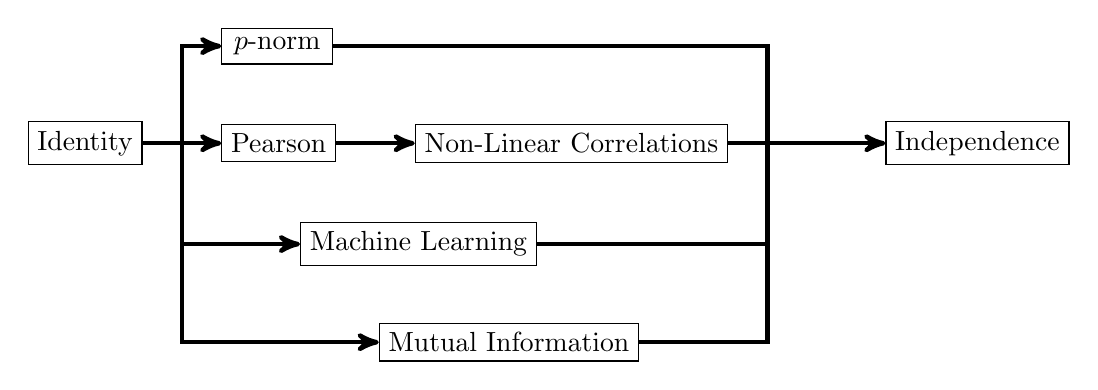
\begin{tikzpicture}
	\node[blocknode] (identity) {Identity};
	\node[blocknode, right = 1 of identity.east] (pearson) {Pearson};
	\node[blocknode, above right = 1 and 1 of identity.east] (pnorm) {$p$-norm};
	\node[blocknode, below right = 1 and 2 of identity.east] (ml) {Machine Learning};
	\node[blocknode, below right = 1 and 1 of ml.west] (mutual) {Mutual Information};
	\node[blocknode, right = 1 of pearson.east] (nonlinear) {Non-Linear Correlations};
	\node[blocknode, right = 2 of nonlinear.east] (independence) {Independence};

	\node[coordinate, right = 0.5 of identity.east] (dummy1) {};
	\node[coordinate, left = 1.5 of independence.west] (dummy2) {};

	\draw[graphedge,-] (identity.east) |- (dummy1.west);
	\draw[graphedge,->] (dummy1.east) |- (pnorm.west);
	\draw[graphedge,->] (dummy1.east) |- (pearson.west);
	\draw[graphedge,->] (dummy1.east) |- (ml.west);
	\draw[graphedge,->] (dummy1.east) |- (mutual.west);
	\draw[graphedge,->] (pearson.east) |- (nonlinear.west);
	\draw[graphedge,-] (pnorm.east) -| (dummy2.west);
	\draw[graphedge,-] (nonlinear.east) -| (dummy2.west);
	\draw[graphedge,-] (ml.east) -| (dummy2.west);
	\draw[graphedge,-] (mutual.east) -| (dummy2.west);
	\draw[graphedge,->] (dummy2.east) |- (independence.west);
\end{tikzpicture}


	\caption{Diffrent similarities}
\end{figure}

\section{From similarity to subspace}
Based on the combined similarity it is possible to calculate subspaces. It is possible to calculate distances between all pairs of dimensions, because of the nature of subspaces. So it is important to find groups in this $\card{D}^2$ relations highly efficient.

Next, I want to discuss how subspaces are formed. Two dimenions should be contained in the subspaces, when they are similar. This can be expressed by a threshold $p_t \in [0,1]$, which the combined similarity should have. By stripping down the similarity matrix to a binary matrix, the dimenions form a graph. This speeds up the calculation, because it allows fast set operations and memory effective management. Because the most data sets have very different dimensions, the number of edges should be low.

Another important attribute of subspaces is that all contained dimenions are similar to each other. This attribute is already described as clique. Because the graph is dense it has a low degeneracy $d \in \set{N}_0$. So, the cliques can be calucated in $\mathcal{O}(d \cdot (\card{D} - d) \cdot 3^{\frac{d}{3}})$ by using \cite{listingCliques}. Because the cliques forms the subspaces, this is the complete algorithm for converting the combined similarity to subspaces.

\section{Optimize graph structure}
A core problem of strict clique searchers is the heavy fragmentation if only one edge missing. Figure~\ref{subfig:opt_graph1} shows an example where the nodes semi clique $\left\{1,2,3,4\right\}$ is splitted into two cliques because of the absence of the edge $(1,3)$. For some applications it could be helpful to add this edge to the graph and join the two cliques into one. The first method to do it is the utilyzation a distance graph:
\begin{envdef}[Strict Distance Graph]
	Given a graph $G=(V,E)$ and a distance $n \in \set{N}_0$, the strict distance graph $G^n=(V,E^n)$ is give by:
	\begin{align}
		E^0 &= \left\{ (v,v) \in V^2 \right\}\\
		E^i &= \left\{ (v_0,v_2) \in V^2 \mid \exists v_1 \in V : (v_0,v_1) \in E^{i-1}, (v_1,v_2) \in E \right\}, \quad \forall i>0
	\end{align}
\end{envdef}
\begin{figure}
	\caption{Different subspaces from different graph preprocessing}
	\label{fig:opt_graph}
	\centering
	\subfloat[\label{subfig:opt_graph1}Too many subspaces]{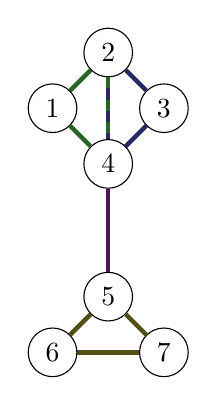
\begin{tikzpicture}
	\node[graphnode] (1) {1};
	\node[graphnode] (2) [above right of=1] {2};
	\node[graphnode] (3) [below right of=2] {3};
	\node[graphnode] (4) [below right of=1] {4};
	\node[graphnode] (5) [below=30pt of 4] {5};
	\node[graphnode] (6) [below left of=5] {6};
	\node[graphnode] (7) [below right of=5] {7};

	\path[graphedge, color=colcontrast]
		(1) edge (2)
			edge (4)
	;

	\path[graphedge, color=colcontrast2]
		(3) edge (2)
			edge (4)
	;

	\path[graphedge, color=colcontrast, dash pattern=on 4pt off 4pt]
		(2) edge (4)
	;

	\path[graphedge, color=colcontrast2, dash pattern=on 4pt off 4pt, dash phase=4pt]
		(2) edge (4)
	;

	\path[graphedge, color=colcontrast3]
		(4) edge (5)
	;

	\path[graphedge, color=colcontrast4]
		(5) edge (6)
			edge (7)
		(6) edge (7)
	;
\end{tikzpicture}

}
	\hfill
	\subfloat[\label{subfig:opt_graph2}Simple graph distance]{\input{figures/graph2.tex}}
	\hfill
	\subfloat[\label{subfig:opt_graph3}Filtered distance with $\alpha=\frac23$]{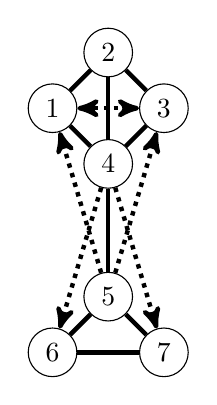
\begin{tikzpicture}
	\node[graphnode] (1) {1};
	\node[graphnode] (2) [above right of=1] {2};
	\node[graphnode] (3) [below right of=2] {3};
	\node[graphnode] (4) [below right of=1] {4};
	\node[graphnode] (5) [below=30pt of 4] {5};
	\node[graphnode] (6) [below left of=5] {6};
	\node[graphnode] (7) [below right of=5] {7};

	\path[graphedge]
		(2) edge (1)
			edge (3)
		(4) edge (1)
			edge (2)
			edge (3)
			edge (5)
		(5) edge (6)
			edge (7)
		(6) edge (7)
	;

	\path[graphedge, dotted]
		(1) edge[<->] (3)
		(5) edge[->] (1)
			edge[->] (3)
		(4) edge[->] (6)
			edge[->] (7)
	;
\end{tikzpicture}

}
	\hfill
	\subfloat[\label{subfig:opt_graph4}Bidirectional filtered distance with $\alpha=\frac23$]{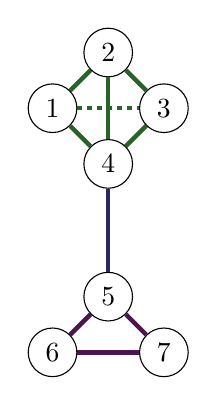
\begin{tikzpicture}
	\node[graphnode] (1) {1};
	\node[graphnode] (2) [above right of=1] {2};
	\node[graphnode] (3) [below right of=2] {3};
	\node[graphnode] (4) [below right of=1] {4};
	\node[graphnode] (5) [below=30pt of 4] {5};
	\node[graphnode] (6) [below left of=5] {6};
	\node[graphnode] (7) [below right of=5] {7};

	\path[graphedge, color=colcontrast]
		(2) edge (1)
			edge (3)
			edge (4)
		(4) edge (1)
			edge (3)
	;

	\path[graphedge, color=colcontrast, dotted]
		(1) edge (3)
	;

	\path[graphedge, color=colcontrast2]
		(4) edge (5)
	;

	\path[graphedge, color=colcontrast3]
		(5) edge (6)
			edge (7)
		(6) edge (7)
	;
\end{tikzpicture}

}
\end{figure}
Because it does not make any sense to forget about the given edges when calcuating higher distances, the definition of the joined distance graph ist more useful:
\begin{envdef}[Joined Distance Graph]
	Given a graph $G=(V,E)$ and a distance $n \in \set{N}_+$, the joined distance graph $G^{\overline{n}}=(V,E^{\overline{n}})$ is definied as followed:
	\begin{equation}
		E^{\overline{n}} = \bigcup_{i=1}^n E^i
	\end{equation}
\end{envdef}
Using the joined distance graph fixes the problem, but does not produce the desired result. As seen in Figure~\ref{subfig:opt_graph2}, it attaches to many new vertices to the cliques and make the results unusable. The reason is that it does not count the strenght of the connection in the exisiting graph and so it creates some edges to weakly connected vertices. A messure for the connection rate between two vertices can be calculated by the following equation:
\begin{envdef}[Connection Rate]
	Given a graph $G=(V,E)$ and two vertices $v_1,v_2 \in V$, the connection rate $r_G(v_1,v_2) \in \left[0,1\right]$ can be calcuated by the relation of connected to all neighbors of $v_1$:
	\begin{equation}
		r_G(v_1,v_2) = \frac{
			\card{ \left\{ v \in V \mid (v_1, v) \in E \right\} \cap \left\{ v \in V \mid (v,v_2) \in E \right\} }
		}{
			\card{ \left\{ v \in V \mid (v_1, v) \in E \right\} }
		}
	\end{equation}
\end{envdef}
Please notice that the connection rate is not symmetric. To honor the connection rate of the vertices, I use a filtered strict distance graph:
\begin{envdef}[Filtered Strict Distance Graph]
	Given a graph $G=(V,E)$, a distance $n \in \set{N}_+$ and a filter rate $\alpha \in \left[0,1\right]$, the filtered strict distance graph $G_\alpha^n=(V,E_\alpha^n)$ is definined as followed:
	\begin{equation}
		E_\alpha^n = \left\{ (v_1,v_2) \in E^n \mid r_{G^{n-1}}(v_1,v_2) \geq \alpha \right\}
	\end{equation}
\end{envdef}
The joined filtered graph, that considers all distances up to a given value, is definied analog:
\begin{envdef}[Filtered Joined Distance Graph]
	Given a graph $G=(V,E)$a distance $n \in \set{N}_+$ and a filter rate $\alpha \in \left[0,1\right]$, the filtered joined distance graph $G_\alpha^{\overline{n}}=(V,E_\alpha^{\overline{n}})$ is definied as followed:
	\begin{equation}
		E_\alpha^{\overline{n}} = \bigcup_{i=1}^n E_\alpha^i
	\end{equation}
\end{envdef}
The filtered joined distance graph is not bidirectional. This leads the problem that there are unidirectional edges that are not usable for our result. As Figure~\ref{subfig:opt_graph3} shows, the weakly connected nodes are connected to the semiclique whereas the semiclique is not connected to the satallites. The inter semiclique edges are bidirectional. Based on this fact, a bidirectional graph can be constructed:
\begin{envdef}[Bidirectional Joined Filtered Distance Graph]
	Given a graph $G=(V,E)$, a distance $n \in \set{N}_+$ and a filter rate $\alpha \in \left[0,1\right]$, the bidirectional joined filtered graph $\tilde{G}_\alpha^{\overline{n}}=(V,\tilde{E}_\alpha^{\overline{n}})$ is defined by the subset of the bidirectional edges of the joined filtered graph:
	\begin{equation}
		\tilde{E}_\alpha^{\overline{n}} = \left\{ (v_1,v_2) \in V^2 \mid (v_1,v_2),(v_2,v_1) \in E_\alpha^{\overline{n}} \right\}
	\end{equation}
\end{envdef}
As shown on Figure~\ref{subfig:opt_graph4} this method successfully adds inter semiclique edges to join them to cliques without creating senseless connections or resulting in informaion loosage. It is important that the graph refinement does not slow down the entire process on big data. In other words, it must not have a higher complexity class. Because the distance parameter $n$ is only used for graph fixing and should not depend on the input size, the following theorem can be shown:

\begin{algorithm}
	\KwData{Vertex $v$}
	\KwData{Graph $G$}
	\KwData{Threshold $t$}
	\KwResult{New neighbors $N$}

	\SetKwFunction{CalcConnectionRate}{calcConnectionRate}
	\SetKwFunction{GetNeighbors}{getNeighbors}

	\Begin{
		\tcc{Search all candidates}
		$C$ $\leftarrow$ $\{\}$\;
		\For{$w \in \GetNeighbors{$v$}$}{
			$C$ $\leftarrow$ $C \cup \GetNeighbors{$w$}$\;
		}

		\BlankLine
		\tcc{Check all candidates}
		$N$ $\leftarrow$ $\{\}$\;
		\For{$c \in C$}{
			\If{$\CalcConnectionRate{$v$, $c$} \geq t \wedge \CalcConnectionRate{$c$, $v$} \geq t$}{
				$N$ $\leftarrow$ $N \cup \{c\}$\;
			}
		}
	}
	\caption{extendNeighbors}
\end{algorithm}

\begin{algorithm}
	\KwData{Graph $G$}
	\KwData{Distance $d$}
	\KwData{Threshold $t$}
	\KwResult{Refined Graph $G_r$}

	\SetKwFunction{ExtendNeighbors}{extendNeighbors}

	\Begin{
		$G_r$ $\leftarrow$ $G$\;
		\For{i=2 \emph{\KwTo} $d$}{
			$G_n$ $\leftarrow$ $()$\;
			\For{$v \in G_r$}{
				$G_n$ $\leftarrow$ $G_n \concat \ExtendNeighbors{$v$, $G_r$, $t$}$\;
			}
			$G_r$ $\leftarrow$ $G_n$\;
		}
	}
	\caption{refineGraph}
\end{algorithm}

\begin{envtheo}
	The graph refinement can be done in $\mathcal{O} ( \card{V}^2 )$ when choosing a fixed distance parameter $n \in \set{N}_+$.
\end{envtheo}
\begin{proof}
	To graph will generated from the graph with the distance $n-1$ where a distance of $1$ is the input graph. Every of this rounds contains two steps. Step one is the calculation of the connection rates, which can be done in $\mathcal{O} ( \card{V}^2 )$. This assumes that data structures are used that can answert the question ``Is vertix $v_1$ connceted to $v_2$?'' in $\mathcal{O} ( 1 )$. The second calculation step is the construction of the new neighborhood for every node. Assuming that you use $\mathcal{O} ( 1 )$ set operations, this can be done for all vertices in $\mathcal{O} ( \card{V}^2 )$. This results in a total cost per round of $\mathcal{O} ( \card{V}^2 )$ and a total algorithm cost of $\mathcal{O} ( n \cdot \card{V}^2 ) = \mathcal{O} ( \card{V}^2 )$.
\end{proof}

\section{Algorithm Summary}
\begin{algorithm}
	\KwData{Dimension $d$}
	\KwData{Binsize $s$}
	\KwResult{Bins $B$}

	\SetKwData{Undef}{undef}

	\SetKwFunction{Sort}{sort}

	\Begin{
		$B$ $\leftarrow$ $()$\;
		$d_s$ $\leftarrow$ \Sort{$d$}\;
		$x$ $\leftarrow$ \Undef\;
		$b$ $\leftarrow$ $()$\;
		\For{$x \in d_s$}{
			\If{$|B| \geq s \wedge x \neq l$}{
				$B$ $\leftarrow$ $B \concat b$\;
				$b$ $\leftarrow$ $()$\;
			}
			$b$ $\leftarrow$ $B \concat x$\;
			$l$ $\leftarrow$ $x$\;
		}
		\If{$|b| \neq 0$}{
			$B$ $\leftarrow$ $B \concat b$\;
		}
	}
	\caption{buildBins}
\end{algorithm}

\begin{algorithm}
	\KwData{Dataset $D$}
	\KwData{Threshold $p_t$}
	\KwData{Graph distance $p_d$}
	\KwData{Threshold of the graph connection rate $p_c$}
	\KwResult{Subspaces $S$}

	\SetKwFunction{BuildBins}{buildBins}
	\SetKwFunction{CalcMeanValues}{calcMeanValues}
	\SetKwFunction{CalcStddevValues}{calcStddevValues}
	\SetKwFunction{CalcVarValues}{calcVarValues}
	\SetKwFunction{CoVar}{coVar}
	\SetKwFunction{DimSimilarity}{dimSimilarity}
	\SetKwFunction{RefineGraph}{refineGraph}
	\SetKwFunction{SearchCliques}{searchCliques}

	\Begin{
		\tcc{Pre calculate aggregates}
		$D_m$ $\leftarrow$ \CalcMeanValues{$D$}\;
		$D_v$ $\leftarrow$ \CalcVarValues{$D$, $D_m$}\;
		$D_s$ $\leftarrow$ \CalcStddevValues{$D_v$}\;

		\BlankLine
		\tcc{Build grid}
		$D_g$ $\leftarrow$ $()$\;
		\For{$d \in D$}{
			$D_g$ $\leftarrow$ $D_g \concat$ \BuildBins{$d$, $\sqrt{|D|}$}\;
		}

		\BlankLine
		\tcc{Build graph}
		\For{$(d_1,m_1,s_1,g_1) \in (D,D_m,D_s,D_g)$}{
			$n$ $\leftarrow$ $\{\}$\;
			\For{$(d_2,m_2,s_2,g_2) \in (D,D_m,D_s,D_g)\setminus\{(d_1,m_1,s_1,g_1)\}$}{
				$x_1$ $\leftarrow$ $\frac{\CoVar{$d_1$, $d_2$, $m_1$, $m_2$}}{s_1 \cdot s_2}$\;
				$x_2$ $\leftarrow$ \DimSimilarity{$g_1$, $g_2$}\;
				\If{$x_1 \cdot x_2 \geq p_t$}{
					$n$ $\leftarrow$ $n \cup \{d_2\}$\;
				}
			}
			$G$ $\leftarrow$ $G \concat n$\;
		}

		\BlankLine
		\tcc{Refine graph}
		$G_r$ $\leftarrow$ \RefineGraph{$G$, $p_d$, $p_c$}\;

		\BlankLine
		\tcc{Search cliques (which are our subspaces)}
		$S$ $\leftarrow$ \SearchCliques{$G_r$}\;
	}
	\caption{calcSubspaces}
\end{algorithm}


\chapter{Implementation}
For the researcher who want only get a described complexity it is sufficient to use a favorite programming languge or DBMS. But if you want to handle big data before getting to old, it is important to choose the right tools and think about some implementation details. In this chapter I want to descibe and explain my choices and would like to give you some impressions about the implementation process. Some but not all strategies can also be used for other algorithms and may be used for some other work too. I will finish the chapter with some ideas about future improvements.

\section{Choosing a programming language}
To express the designed algorithm and let the computer do the job it is necessary to write some source code. There are dozend different programming languages out there and every language has its own pros and cons.

A simple and very comfortable choice is a language with a good buildin runtime library.\footnote{What ``good'' means in this context depends on the algorithm that you want to implement and the operations you need.} Python or Matlab is a good choice. Please notice that SQL or other database bound languages are not very portable and suffer when it comes to debugging and flexibility. If the language provided a embedded mathematic system like Matlab, it is easy to map the theoretical terms to the language. Matrix support makes it easy to handle big amounts of data. The key feature of the language should be syntax that does not produce much boiler plate. This is one point where script languages are very good, but lanuages like Java are not. C++ provides a short syntax for many things, but suffers like many other compiled langues when you want a comfortable environment. Typesafety is another point that can be useful because it allowes you to tackle many bugs before you waste your time for runtime tests.

The next point is a good library support for things that the choosen language does not provide. Matrix operations require a special library, escecially if you want to invert or decomposit them. High precision floating point operations and big integer calculation needs a different library. Parsing, code managment or special IO operations is another topic. Also notice that I don't mean the standard library. A well tested and documented library is required. For example NumPy if you use Python.

In addition to the things you as the author and primary user of the implementation finds useful are the problems your team or the consumers need. An exotic language\footnote{Don't know what I mean? Go and find something about APL} may be very cool but if nobody can read your code, your research result doesn't help someone. This does not mean that you have to stuck in old good Java or COBOL, but it means that you have to think about the innovation you want to use. Also think about portability, future development and safety of the language. Safety is important if you don't want to risk the data of your institution or the consumers. You may think that the implementation is only for internal tests but if your results are good it can be the case that your code will be published or used by other persons. Even if low level languages can be insecure when doing unchecked memory operations, also interpreted languages have many weaknesses.

You may ask where this all have to do with high perfomance. The simple answer is: nothing. They make your life easier, but do not provide a fast implementation. So the most important point for my work is performance. And this kills the most high level languages, because they do not provide a fine grained control about data allocation, movement and copying. Even the object overhead of languages like Java and naiv C++ is too big. I had to strip down the calculation core to a simple low level core. But I do not want to loose all high level features. In my eyes, there is currently only one languages that provides this schizophrenia: handcrafted and well written C++. I will give you some rules about hints about the language specific methods in the next section.

\section{Special C++ tips}
C++ can be used in many different ways, depending on your background, the interfaces you want to use or have to provide and the attributes your program should have. As most other programming languages out there, C++ is avaiable in different standarts and the compiler and STL support differs. One of the best collections of tips for good programming style is \cite{effectiveCpp}. Furthermore I used the new C++11 standard which brings makes many code sections easier to read and more C++ stylish rather than C based. It also avoids many boiler blade an manual memory management. Templates may be the most hated but most also most loved and most essential features of C++. I used them when I find it useful. Some calculations are written in C style because in some cases, the object overhead was to high. Because of the usage of new C++11 featues, the resulting code only compiles with newer versions of GCC and Clang. Microsoft and Intel compilers are not suppported at the time of the writing.

\section{Avoiding reinventing the wheel}
The STL already provides useful tools that makes programmers life much easier. But it does not provide high level thread operations like fork and join, system operations like memory mapped IO and fast a fast parser library. C++ has a special collection of well designed and reviewed libraries that are note yet a part of the STL: The Boost C++ Libraries. They provide two of the three libraries I was looking for -- the Boost Interprocess library, which implements memory mapped IO and the Spirit V2 library which is a special set of function and templates for parser writing. For high level multi core operations I use another well known library: the TBB, which is designed and published by Intel. All libraries are open source and free which enables researcher to use them for their work.

\section{The low level data backend}
In the field of data processing and data mining, many algorithms where build on top of exisiting server driven databases. This has many benefits. In many cases, the data that should be analyzed already exists in this databases in a normalized form and is supplied by fresh data. Because of the nature of feature selection, column stores are than row oriented stores. They provide a cache local access to data of different dimensions and reduces the processing overhead. The main drawback of the most server driven data stores is the performance when using complex algorithms.\footnote{This may change in the next few years when in-memory databases become more prominent and affordable.} Another solution is using an embedded database like SQLite, but they also have too much overhead when accessing raw data. Please consider that the database also provides too many operations that are not needed for this kind of data processing. Only apped and read operations are required, no indices, no aggregations, no write, modify and delete.

This brings me to the question why I need a backend for data storage. In the current situation, most researchers don't have systems with enough main memory to hold the complete data. So it is important that they have a backend that can easely page out data to the disc or SSD. This should also be combined with low overhead. So sequencial loading on demand is not an option. Another problem is that the application programmer cannot easely determine, when the system runs out of memory, because the OS swaps out data on its own discretion. An old but very wise advice of OS designers is, that the kernel always has better information about the entire system than every user program. So why not let the kernel do the job? So I decided to just use plain arrays for column representation and memory map them from a file. So the kernel can load them or page them out if necessary. For better managment and better append operations, the columns are defided into fixed size segments. The segments and the column metadata like size and name are managed by the Boost Interprocess Library, which uses a trees to manage a string to pointer mapping.

As shown in chapter~\ref{chap:algodesign} the algorithm needs a graph structure. An append only graph can mapped to a column store by utilizing two columns and encode each vertex as an unique, continous, unsigned integer. One column is called the neighbor column and stores the appended list of all neighbors of all vertices. The other column is called the index column stores the split points of the neighbor column. To get back the neighbors of an vertex $v$, just output the neighbor column from the index that is written in the in index column at position $v$ to the index that is written at position $v+1$.

Maps for precalcuated metadata can also be mapped to column stores by storing key value tuples and rebuilding the hash index when loading the map. This does not have perfomance impact because the algorithm only need a small fixed number of metadata per dimension.


\chapter{How to beat the system}\label{chap:beat}
GraBaSS only uses the relationship between two dimensions to build up a graph and find cliques which forms the subspaces. It is possible, that this pairwise approach does not find higher order dependencies. In this case, there are subspaces that are not found by GraBaSS or subspaces that do not reach their maximum size. The pairwise approach was not only chosen for performance but also because it is sufficient for the most data set. In this chapter, I will show how a higher order data set could look like, why this kind is not very common and how to handle them.

\section{Constructing a special dataset}\label{sec:constr}
In mathematical terms, higher order dependencies exists because of the following fact:
\begin{envtheo}\label{theo:lowdep}
	Given three dimensions $X$, $Y$ and $Z$, which satisfy the following requirement:
	\begin{equation}\label{equ:low_independency}
		\begin{aligned}
			\prob{X = x, Y = y} &= \prob{X = x} \prob{Y = y},\quad & \forall (x,y) &\in X \times Y \\
			\prob{Y = y, Z = z} &= \prob{Y = y} \prob{Z = z},\quad & \forall (y,z) &\in Y \times Z \\
			\prob{Z = z, X = x} &= \prob{Z = z} \prob{X = x},\quad & \forall (z,x) &\in Z \times X
		\end{aligned}
	\end{equation}
	there can cases where $\exists (x,y,z) \in X \times Y \times Z$:
	\begin{equation}
		\prob{X = x, Y = y, Z = z} \neq \prob{X = x} \prob{Y = y} \prob{Z = z}
	\end{equation}
	So condition~\ref{equ:low_independency} is not sufficient for independence of the given dimensions.
\end{envtheo}
\begin{proof}
	See example described below.
\end{proof}

To illustrate the situation explained in theorem~\ref{theo:lowdep}, consider the following a dataset, that is made of many random points $(x, y, z) \in \left[0, 1\right)^3$, that satisfy the following constraint:
\begin{equation}\label{eq:beat}
	(x + y + z) \bmod 1 = 0
\end{equation}
The points are uniform distributed if you project them on one or two dimensions. But if you calculate the three dimensional distribution, the points do not show a uniform distribution. (see Figure~\ref{fig:beat}). Because the generated points have two degrees of freedom, the two dimensional distribution test will fail. It is also possible to generate datasets with even more degrees of freedom using the same technique.\footnote{You may not be able to imagine datasets with more than three dimensions. For 4 dimensions, you find some help: \url{http://crepererum.github.io/brain4D/\#constructed}}
\begin{figure}
	\caption{Situation described in Equation~\ref{eq:beat}}
	\label{fig:beat}
	\subfloat[\label{subfig:beat1}1D views]{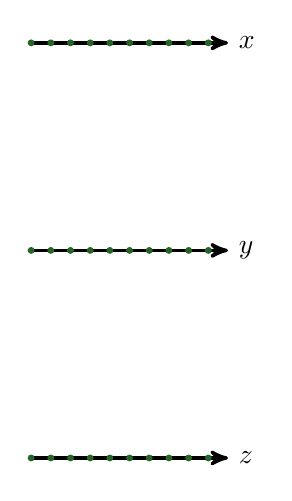
\begin{tikzpicture}[scale = 5.0]
	\foreach \name [count=\d from 0] in {x,y,z} {
		\begin{scope}[yshift=-\d*15]
			\begin{scope}[scale=0.5]
				\draw[axis] (0,0) -- (1,0) node[right]{$\name$};
				\foreach \x in {0,...,9} {
					\fill[colcontrast] (\x/10,0) circle(0.5pt);
				}
			\end{scope}
		\end{scope}
	}
\end{tikzpicture}

}
	\hfill
	\subfloat[\label{subfig:beat2}2D views]{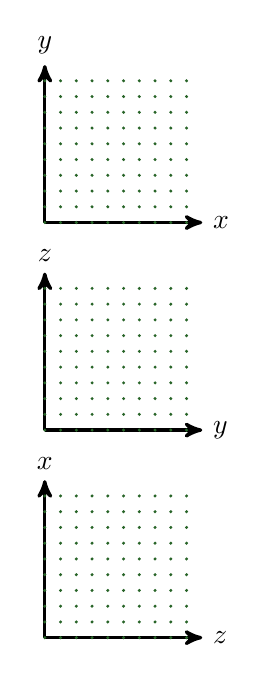
\begin{tikzpicture}[scale = 5.0]
	\foreach \namefirst/\namesecond [count=\d from 0] in {x/y,y/z,z/x} {
		\begin{scope}[yshift=-\d*15]
			\begin{scope}[scale=0.4]
				\draw[axis] (0,0) -- (1,0) node[right]{$\namefirst$};
				\draw[axis] (0,0) -- (0,1) node[above]{$\namesecond$};
				\foreach \x in {0,...,9} {
					\foreach \y in {0,...,9} {
						\fill[colcontrast] (\x/10,\y/10) circle(0.3pt);
					}
				}
			\end{scope}
		\end{scope}
	}
\end{tikzpicture}

}
	\hfill
	\subfloat[\label{subfig:beat3}3D view]{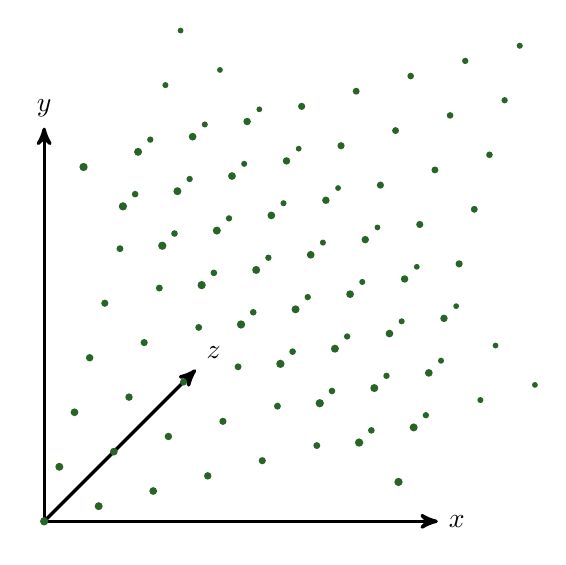
\begin{tikzpicture}[scale = 5.0]
	\begin{scope}[scale=1.0]
		\draw[axis] (0,0,0) -- (1,0,0) node[right]{$x$};
		\draw[axis] (0,0,0) -- (0,1,0) node[above]{$y$};
		\draw[axis] (0,0,0) -- (0,0,-1) node[above right]{$z$};
		\foreach \x in {0,...,9} {
			\foreach \y in {0,...,9} {
				\pgfmathsetmacro{\z}{mod(\x+\y,10)}
				\fill[colcontrast] (\x/10,\y/10,-\z/10) circle(0.3pt-0.1pt*\z/10);
			}
		}
	\end{scope}
\end{tikzpicture}

}
	\hfill
\end{figure}

The problem occurs every time, when the dataset contains a subspace with $n \in \set{N}_+$ Dimensions but $m \in \left\{1,\dots,n-1\right\}$ degrees of freedom. Furthermore the dependency of each dimension on the degrees of freedom has to be equal, so no relation is visible in two dimensional projections. Especially the last condition is uncommon when looking at real world data sets.

\section{Handling this issue}
For data sets which has dimensions described in theorem~\ref{theo:lowdep}, I will propose a simple method to handle them. To get a good performance on high dimensional datasets, it is not possible to check all higher order dependencies. Because the described problem occurs when the degrees of freedom are not aligned with the dimensions, a transformation of the dataset to the degrees of freedom would help. PCA is a well known method which finds such transformations. As shown in \cite{pca}, a PCA can be computed in $O ( \card{D}^2h + \card{D}^2\card{N} )$ where $h$ is the number of degrees of freedom. If the dependencies of the dimension are formed by a near-linear process, PCA will find them. The result of the transformation can be used as input for GraBaSS. The isolated subspaces and the transformation found by PCA together explain the relation between dimensions. If there is any prior knowledge about the data set, it can be used to find such problematic dimensions. Note, that PCA can also be applied to subspaces before and after using GraBaSS, where the pre-analysis subspaces can be extracted by using expert knowledge.


\chapter{Datasets}
High dimensional datasets are not a very common research topics. In this chapter I will describe some data sources and possible applications of the described algorithm. I also show some interpretations of subspaces in different datasets and some failed approaches of finding them. To get, isolate and preprocess the data I've used some scripts. Because I think open research should not only contain open publications but also open data sources, you can find the scripts and some notes about them online.\footnote{\url{https://github.com/crepererum/GSD}} Should you have some questions, find a bug or want to contribute, feel free to use the issue tracker or file a pull request.

\section{Drug Database}
A source of high dimensional data is the list of ingredients of drugs. They collect important information about common combination of substances because one ingredient requires another, e.g. alcohol is a solvent for many chemicals. Common combinations can also be formed by combined substances that are used in drugs because manufactures produce them as a base for their product or because they act as a reseller for premixed drugs. The data set also contains information about chemicals that are never used together because they react with each other or because it does not make sense in terms of usability.

I hoped to find some public drug data bases containing drugs registered in Germany or in the EU. But this was not the case. Either they were only usable via a very limited interface or it would cost me a enormous amount of money to buy a license. Since the open data movement in USA has a very long tradition, it was easy to find an American drug database, that is easy to parse and provides a huge data collection.\footnote{\url{http://dailymed.nlm.nih.gov/dailymed/downloadLabels.cfm}} The entire data set contains \num{24094} drugs and \num{4139}. Figure~\ref{fig:drugs} visualizes a spectrum of this dataset, where rows act as drugs and image columns describe if a specific drug contains a specific substance. The most common ingredients in this data are:
\begin{itemize}
	\item water
	\item glycerin
	\item titanium dioxide
	\item propylene glycol
	\item dimethicone
\end{itemize}

\begin{figure}
	\includegraphics[height=\textheight,keepaspectratio]{drugs}
	\caption{drugs spectrum}
	\label{fig:drugs}
\end{figure}

To convert this data to a legal input data set, it is processed as followed: The only preprocessing that is done is to reduce the ingredients to their lower case text because the data set contains the same ingredients written in different combinations of lower and upper case letters. After the case normalization build a list of all ingredients in all drugs and bring them into a fixed order. Every ingredient forms one dimension. Then build a binary vector for every drug in the database where $1$ describes that a ingredient is contained in the drug and $0$ if this is not the case. I provide a parser and converter for this kind of data.

GraBaSS is used with $t_e = 0.25$, $t_n = 0.65$ and $d = 3$. It extracts many subspaces, that describe rare combinations, that are used in some natural products. The listed substances are also natural, e.g. leafs, flowers and roots. Because the ingredients are so uncommon, they form subspaces when only used together only a few times. Trying to eliminate this substances is not possible without loosing most of the data set because there are only a few substances that are very common and many that are uncommon.

Some examples for more usable subspaces are:
\begin{itemize}
	\item boron, bromine, lithium, magnesium, manganese, potassium, sodium, strontium
	\item alanine, asparagine, cysteine, histidine, ornithine, threonine
\end{itemize}

ENCLUS extracted very small subspaces. When increasing $\epsilon$, the algorithm does not finish within hours because the data set is too large. So I got no usable results.


\chapter{Conclusion and further research}
Feature selection is an important task when analyzing data. It helps to understand relationships of attributes, speeds up further analysis tasks and handles the curse of dimensionality. Big data sets of today and the next years require an efficient way and parallel algorithms that provide solid results. With GraBaSS, I developed one small piece for the data processing of the next years. It is not only a algorithm, but also a framework and an illustration of ideas that can used by other researcher. It outperforms other approaches when in comes to calculation time and provides clearer, in some cases even better results. The implementation uses optimizations to archive high performance and low memory footprint.

But GraBaSS and its implementation are not perfect. The chosen similarity is suitable for all tasks, especially when high contrast is required. The realization in C++ does not use GPUs or other accelerators like FGPAs and is not scalable about multiple computers. To archive this the first one, an OpenCL based implementation and further memory optimization could help. The latter one requires a solid foundation of network code, error detection and load balancing. Heterogeneous architectures makes this task even more complicated. A high performance, in-memory database which provides a generic interface for this kind of algorithm would be required. Another part, which is not researched very well are incremental algorithms, which do not require a full recalculation when new data points or even new dimensions are added to the data set.

So there are many topics left for research especially because data set size increases and real time information becomes more important. I believe that this is not my last work in this field and I hope to provide a small piece for better technology that may help other people in a wide range of tasks, today and in future times. 


\appendix

\backmatter

\listoffigures

\listofalgorithmes

\printnomenclature

\printglossaries

\cleardoublepage
\phantomsection
\addcontentsline{toc}{chapter}{Bibliography}
\printbibliography

\end{document}

